\documentclass[c,18pt]{beamer}
\listfiles

\mode<presentation>
{
  \usetheme[deutsch,titlepage0]{KIT}
  \setbeamercovered{transparent}
  \setbeamertemplate{enumerate items}[ball]
}
\usepackage[utf8]{inputenc}
\date{23.10.2018}

\newlength{\Ku}
\setlength{\Ku}{1.43375pt}

\usepackage{templateSlide/exercises}
\usepackage[java]{code}

\makeatletter
\def\input@path{{uebungsfolien/}}
\graphicspath{{uebungsfolien/}}
\makeatother

%% title slide
\title[Übung 01: Einstieg in die Informatik und algorithmische]
  {Übung 01: Einstieg in die Informatik und algorithmische \\ Mathematik}
\subtitle{Albert Mink | Wintersemester 2018/2019}

\author[Albert Mink, ]{KIT}

\AuthorTitleSep{\relax}

\institute[Institut für Angewandte und Numerische Mathematik (IANM)]{Institut für Angewandte und Numerische Mathematik}

\TitleImage[width=\titleimagewd]{logos/KIT-Titel}
\logo{
\includegraphics{logos/lbrg_logo}}

%%%%%%%%%%%%%%%%%%%%%%%%%%%%%%%%%%%%%%%%%%%%%%%%%%%%%%%%%%%%%%%%%%%%%%%%
% Document
%%%%%%%%%%%%%%%%%%%%%%%%%%%%%%%%%%%%%%%%%%%%%%%%%%%%%%%%%%%%%%%%%%%%%%%%
\begin{document}
\begin{frame}
  \maketitle
\end{frame}
%%%%%%%%%%%%%%%%%%%%%%%%%%%%%%%%%%%%%%%%%%%%%%%%%%%%%%%%%%%%%%%%%%%%%%%%

\begin{frame}
  \frametitle{Arbeitsblatt 1}%
%\tableofcontents[hideallsubsections]
\end{frame}
%TODO listings add linerange

%%%%%%%%%%%%%%%%%%%%%%%%%%%%%%%%%%%%%%%%%%%%%%%%%%%%%%%%%%%%%%%%%%%%%%%%
%%%%%%%%%%%%%%%%%%%%%%%%%%%%%%%%%%%%%%%%%%%%%%%%%%%%%%%%%%%%%%%%%%%%%%%%
\section{Wiederholung}\label{K:wdh}
\begin{frame}
  \frametitle{\ref{K:wdh} Wiederholung}%
\tableofcontents[current]
\end{frame}


%%%%%%%%%%%%%%%%%%%%%%%%%%%%%%%%%%%%%%%%%%%%%%%%%%%%%%%%%%%%%%%%%%%%%%%%
\def\stitle{Stellenwertsystem}
\subsection{\stitle}\label{S:Stellenwertsystem}
\begin{frame}[fragile]%
  \frametitle{\ref{K:wdh}.\ref{S:Stellenwertsystem} \stitle}%
\medskip

Eine Zahl l\"asst sich in einem Stellenwertsystem zu einer Basis $b$ durch eine Ziffernfolge darstellen, die Basis wird dabei in der Regel als Index gegeben.
Zum Beispiel die Zahl $426_8$, gegeben im Oktalsystem:
\begin{equation*}
426_8 = 4*8^2 + 2*8^1 + 6*8^0 = 256 + 16 + 6 = 278_{10} = 278
\end{equation*}
M\"ochte man nicht in oder von dem Dezimalsystem umrechnen, ist oft dennoch ein Umweg dar\"uber notwendig, au\ss er die Basis des einen Systems ist eine Potenz der Basis eines anderen Systems ($b_1 = b_2^n$).
In diesem Fall lassen sich die Zahlen in Bl\"ocke unterteilen.
Beispiel Bin\"arsystem und Oktalsystem:
\begin{align*}
426_8 \rightarrow \quad & \quad   4 & | & \quad   2 & | & \quad   6 & \\
                        & \quad 100 & | & \quad 010 & | & \quad 110 & \quad \rightarrow 100010110_2
\end{align*}

\end{frame}


%%%%%%%%%%%%%%%%%%%%%%%%%%%%%%%%%%%%%%%%%%%%%%%%%%%%%%%%%%%%%%%%%%%%%%%%
\def\stitle{Grundlagen in Java}
\subsection{\stitle}\label{S:GrundlageninJava}
\begin{frame}[fragile]%
  \frametitle{\ref{K:wdh}.\ref{S:GrundlageninJava} \stitle}%
\medskip

\begin{description}[leftmargin=*,style=nextline]
\item[\textcolor{KITgreen}{\textbf{Datentypen}}]
\item[Ganzzahlige Typen]  \code{byte, short, int, long}
\item[Gleitkomma Typen]   \code{float, double}
\item[Zeichen]            \code{char, String}
\item[Boolscher Typen]    \code{boolean}
\end{description}
\medskip

\begin{description}[leftmargin=*,style=nextline]
\item[\textcolor{KITgreen}{\textbf{Variablen}}]
\item[Deklaration] \code{double x;}
\item[Definition] \code{int n = -1;}
\item[Wertzuweisung] \code{int a = n;}
\end{description}

\end{frame}


%%%%%%%%%%%%%%%%%%%%%%%%%%%%%%%%%%%%%%%%%%%%%%%%%%%%%%%%%%%%%%%%%%%%%%%%
\def\stitle{Kompilieren und Ausführen}
\subsection{\stitle}\label{S:CompilierenUexec}
\begin{frame}[fragile]%
  \frametitle{\ref{K:wdh}.\ref{S:CompilierenUexec} \stitle}%
\medskip

Um das Programm Hello World auszuführen werden folgende Schritte auf dem Terminal durchgeführt.

\begin{lstlisting}[style=BASH]
javac HelloWorld.java
java HelloWorld
Hello World!
\end{lstlisting}

\end{frame}


%%%%%%%%%%%%%%%%%%%%%%%%%%%%%%%%%%%%%%%%%%%%%%%%%%%%%%%%%%%%%%%%%%%%%%%%
%%%%%%%%%%%%%%%%%%%%%%%%%%%%%%%%%%%%%%%%%%%%%%%%%%%%%%%%%%%%%%%%%%%%%%%%
\section{Aufgabe 1}
\def\stitle{\theexercise\ - Programmentwicklung}
\section{\stitle}
\begin{frame}%
  \frametitle{\stitle}%
\tableofcontents[current]
\end{frame}


\begin{frame}%
  \frametitle{\stitle}%

\begin{itemize}
\item Wozu dient der Java-Compiler, wozu der Java-Interpreter?
\item Erläutern Sie die Aussage \glqq Java ist plattformunabhängig\grqq.
\end{itemize}

\end{frame}


\begin{frame}[t]%
  \frametitle{\stitle\ Fortsetzung}%
\centering

\includegraphics[width=0.6\textwidth]{\getexercisefolder Java-Kompiler}\\[2em]
\includegraphics[width=0.6\textwidth]{\getexercisefolder C++-Kompiler}

\begin{itemize}
 \item Java-Bytecode ist plattformunabhängig und kann vom Java-Interpreter auf jedem System ausgeführt werden.
 \item C++ Programme können direkt vom Betriebssystem ausgeführt werden, wenn sie für dieses kompiliert wurden.
\end{itemize}

\end{frame}



%%%%%%%%%%%%%%%%%%%%%%%%%%%%%%%%%%%%%%%%%%%%%%%%%%%%%%%%%%%%%%%%%%%%%%%%
%%%%%%%%%%%%%%%%%%%%%%%%%%%%%%%%%%%%%%%%%%%%%%%%%%%%%%%%%%%%%%%%%%%%%%%%
\section{Aufgabe 2}
\def\stitle{\theexercise\ - Literale}
\section{\stitle}
\begin{frame}%
  \frametitle{\stitle}%
\tableofcontents[current]
\end{frame}

\begin{frame}[fragile]%
  \frametitle{\stitle}%


Nachfolgend finden Sie Beispiele von Java-\emph{Literalen}, d.h. von Zeichenfolgen die in einem Java-Quelltext konstante Werte repräsentieren.
Geben Sie jeweils den Datentyp des Literals an.
Mögliche Datentypen sind \code{int}, \code{long}, \code{double}, \code{float}, \code{boolean}, \code{char} und \code{String}.

\begin{center}

\begin{minipage}{0.3\textwidth}
\begin{enumerate}
\item \code{"Hello!"}
\item \code{-156}
\item \code{1E6}
\item \code{" "}
\end{enumerate}
\end{minipage}
\hfill
\begin{minipage}{0.3\textwidth}
\begin{enumerate}
\setcounter{enumi}{4}
\item \code{0.5}
\item \code{'0'}
\item \code{1.5e-1}
\item \code{124f}
\end{enumerate}
\end{minipage}
\hfill
\begin{minipage}{0.3\textwidth}
\begin{enumerate}
\setcounter{enumi}{8}
\item \code{"13"}
\item \code{true}
\item \code{'a'}
\item \code{.2}
\end{enumerate}
\end{minipage}

\end{center}
\end{frame}


% Lösungen
\begin{frame}[fragile]%
  \frametitle{\stitle}%


Die L"osungen lauten:

\begin{center}

\begin{minipage}{0.3\textwidth}
\begin{enumerate}
\item \code{"Hello!"} $\rightarrow$ \code{String}\\
\item \code{-156}     $\rightarrow$ \code{int}\\
\item\code{1E6}       $\rightarrow$ \code{double}\\
\item \code{" "}      $\rightarrow$ \code{String}\\
\end{enumerate}
\end{minipage}
\hfill
\begin{minipage}{0.3\textwidth}
\begin{enumerate}
\setcounter{enumi}{4}
\item \code{0.5}   $\rightarrow$ \code{double}\\
\item \code{'0'}   $\rightarrow$ \code{char}\\
\item \code{1.5e-1}$\rightarrow$ \code{double}\\
\item \code{124f}  $\rightarrow$ \code{float}\\
\end{enumerate}
\end{minipage}
\hfill
\begin{minipage}{0.3\textwidth}
\begin{enumerate}
\setcounter{enumi}{8}
\item \code{"13"} $\rightarrow$ \code{String}\\
\item \code{true} $\rightarrow$ \code{bool}\\
\item \code{'a'}  $\rightarrow$ \code{char}\\
\item \code{.2}   $\rightarrow$ \code{double}\\
\end{enumerate}
\end{minipage}

\end{center}
\end{frame}


\begin{frame}[t]%
  \frametitle{\stitle\, Bsp Programm}%

\lstinputlisting[style=JAVAsmall]
{\getexercisefolder Literale.java}
\end{frame}



%%%%%%%%%%%%%%%%%%%%%%%%%%%%%%%%%%%%%%%%%%%%%%%%%%%%%%%%%%%%%%%%%%%%%%%%
\begin{frame}[t]%
  \frametitle{Aufgabe 2, Beispielprogramm}%
\medskip

\lstinputlisting[style=JAVAsmall]
{grundl-literale/Literale.java}
\end{frame}

%%%%%%%%%%%%%%%%%%%%%%%%%%%%%%%%%%%%%%%%%%%%%%%%%%%%%%%%%%%%%%%%%%%%%%%%
%%%%%%%%%%%%%%%%%%%%%%%%%%%%%%%%%%%%%%%%%%%%%%%%%%%%%%%%%%%%%%%%%%%%%%%%
\section{Aufgabe 3}
\begin{exercise}{Ausdrücke}

\begin{body}
Nachfolgend finden Sie Beispiele von Java-Ausdrücken. Geben Sie jeweils das Ergebnis des Ausdrucks sowie den 
Datentyp des Ergebnisses an. Mögliche Datentypen sind \code|int|, \code|double|, \code|bool|, \code|char| und \code|String|.
\begin{center}
\begin{minipage}{0.3\textwidth}
\begin{itemize}
\item[(a)] \code|12.3 + 1|
\item[(b)] \code|0.5 * 4|
\item[(c)] \code|2.0 / 4.0|
\item[(d)] \code|(2-1.0)/5| 
\item[(e)] \code|14.0 % 5|
\end{itemize}
\end{minipage}
\begin{minipage}{0.3\textwidth}
\begin{itemize}
\item[(f)] \code|3 / 6.0|
\item[(g)] \code|(int) 1.23|
\item[(h)] \code|2 / (int) 3.14|
\item[(i)] \code|1.0 / 4|
\item[(j)] \code|15 % 2|
\end{itemize}
\end{minipage}
\begin{minipage}{0.3\textwidth}
\begin{itemize}
\item[(k)] \code|1>2|
\item[(l)] \code|'a' + 1|
\item[(m)] \code|1 / 2|
\item[(n)] \code|1 == 2|
\item[(o)] \code|(1+1)>1|
\end{itemize}
\end{minipage}
\end{center}
\end{body}

\begin{solution}

\begin{center}
\begin{minipage}{0.3\textwidth}
\begin{itemize}
\item[(a)] $13{,}3$  \\ \code|double|
\item[(b)] $2$       \\ \code|double|
\item[(c)] $0{,}5$   \\ \code|double|
\item[(d)] $0{,}2$   \\ \code|double|
\item[(e)] $4$ ($14 = 2\cdot 5 + \boldsymbol{4}$) \\ \code|double|
\end{itemize}
\end{minipage}
\begin{minipage}{0.3\textwidth}
\begin{itemize}
\item[(f)] $0{,}5$   \\ \code|double|
\item[(g)] $1$ (ganzzahliger Anteil) \\ \code|int|
\item[(h)] $0$               \\ \code|int|
\item[(i)] $0{,}25$  \\ \code|double|
\item[(j)] $1$ ($15 = 7\cdot 2 + \boldsymbol{1}$) \\ \code|int|
\end{itemize}
\end{minipage}
\begin{minipage}{0.3\textwidth}
\begin{itemize}
\item[(k)] \code|false|          \\ \code|bool|
\item[(l)] $98$ (ANSI: `a' = $97$) \\ \code|int|
\item[(m)] $0$  (Ganzzahldivision) \\ \code|int|
\item[(n)] \code|false|      \\ \code|bool|
\item[(o)] \code|true|            \\ \code|bool|
\end{itemize}
\end{minipage}
\end{center}
\end{solution}

\end{exercise}
 %% Java Bsp Code


%%%%%%%%%%%%%%%%%%%%%%%%%%%%%%%%%%%%%%%%%%%%%%%%%%%%%%%%%%%%%%%%%%%%%%%%
\begin{frame}[t]%
  \frametitle{Aufgabe 3, Beispielprogramm (1)}%
\medskip

\lstinputlisting[style=JAVAsmall]
{grundl-ausdruecke/Ausdruecke1.java}
\end{frame}


%%%%%%%%%%%%%%%%%%%%%%%%%%%%%%%%%%%%%%%%%%%%%%%%%%%%%%%%%%%%%%%%%%%%%%%%
\begin{frame}[t]%
  \frametitle{Aufgabe 3, Beispielprogramm (2)}%
\medskip

\lstinputlisting[style=JAVAsmall]
{grundl-ausdruecke/Ausdruecke2.java}
\end{frame}


%%%%%%%%%%%%%%%%%%%%%%%%%%%%%%%%%%%%%%%%%%%%%%%%%%%%%%%%%%%%%%%%%%%%%%%%
%%%%%%%%%%%%%%%%%%%%%%%%%%%%%%%%%%%%%%%%%%%%%%%%%%%%%%%%%%%%%%%%%%%%%%%%
\section{Aufgabe 4}
\begin{frame}[t]%
\medskip

\begin{exercise}{Stellenwertsysteme}
\begin{body}
Bei \emph{Stellenwertsystemen} wird eine Zahl durch eine Folge ${z_n z_{n-1} \dotsb z_1 z_0}$ von \emph{Ziffern} $z_k$ dargestellt. Jedes Stellenwertsystem bezieht sich dabei auf eine bestimmte \emph{Basis} $b$, die man bei Bedarf als Subskript an das Ende der Ziffernfolge schreibt. Für die Ziffern gilt $z_k \in \{0,1,\dotsc,b-1\}$. Eine Ziffernfolge
${z_n z_{n-1} \dotsb z_1 z_0}$ im Stellenwertsystem zur Basis $b$ stellt die Zahl
\[  z_n \cdot b^{n} + z_{n-1} \cdot b^{n-1} + \dotsb + z_1 \cdot b^1 + z_0 \cdot b^0  \]
dar. Wichtige Stellenwertsysteme sind das \emph{Dezimalsystem} ($b = 10$), das \emph{Binärsystem} ($b = 2$), das \emph{Oktalsystem} ($b = 8$) und das \emph{Hexadezimalsystem} ($b = 16$). Geben Sie die Darstellung der folgenden  Binär-, Oktal-, Hexadezimal- und Dezimalzahlen in den jeweils anderen Stellenwertsystemen an. Im Hexadezimalsystem bezeichnen die Buchstaben $\mathrm{A},\mathrm{B}, \dotsc, \mathrm{F}$ die Ziffern $10, 11, \dotsc, 15$.
\begin{center}
\begin{minipage}{0.22\textwidth}
\begin{parts}
\item[(a)] $10_2$
\item[(b)] $1100_2$
\item[(c)] $10101_2$
\item[(d)] $101010_2$
\end{parts}
\end{minipage}
\begin{minipage}{0.22\textwidth}
\begin{parts}
\item[(e)] $27_8$
\item[(f)] $133_8$
\item[(g)] $10_8$
\item[(h)] $77_8$
\end{parts}
\end{minipage}
\begin{minipage}{0.22\textwidth}
\begin{parts}
\item[(i)] $\mathrm{2A}_{16}$
\item[(j)] $10_{16}$
\item[(k)] $\mathrm{FF}_{16}$
\item[(l)] $\mathrm{D1}_{16}$
\end{parts}
\end{minipage}
\begin{minipage}{0.22\textwidth}
\begin{parts}
\item[(m)] $17_{10}$
\item[(n)] $33_{10}$
\item[(o)] $65_{10}$
\item[(p)] $72_{10}$
\end{parts}
\end{minipage}
\end{center}
\end{body}


\begin{solution}
\begin{center}
\begin{minipage}{0.45\textwidth}
\begin{parts}
\item[(a)] $10_2 = 2_8 = 2_{10} = 2_{16}$
\item[(b)] $1100_2 = 14_8 = 12_{10} = \mathrm{C}_{16}$
\item[(c)] $10101_2 = 25_8 = 21_{10} = 15_{16}$
\item[(d)] $101010_2 = 52_8 = 42_{10} = \mathrm{2A}_{16}$
\item[(e)] $27_8 = 10111_2 = 23_{10} = 17_{16}$
\item[(f)] $133_8 = 1011011_2 = 91_{10} = \mathrm{5B}_{16}$
\item[(g)] $10_8 = 1000_2 = 8_{10} = 8_{16}$
\item[(h)] $77_8 = 111111_2 = 63_{10} = \mathrm{3F}_{16}$
\end{parts}
\end{minipage}
\begin{minipage}{0.45\textwidth}
\begin{parts}
\item[(i)] $\mathrm{2A}_{16} = 101010_2 = 52_8 = 42_{10}$
\item[(j)] $10_{16} = 10000_2 = 20_8 = 16_{10}$
\item[(k)] $\mathrm{FF}_{16} = 11111111_2 = 377_8 = 255_{10}$
\item[(l)] $\mathrm{D1}_{16} = 11010001_2 = 321_8 = 209_{10}$
\item[(m)] $17_{10} = 10001_2 = 21_8 = 11_{16}$
\item[(n)] $33_{10} = 100001_2 = 41_8 = 21_{16}$
\item[(o)] $65_{10} = 1000001_2 = 101_8 = 41_{16}$
\item[(p)] $72_{10} = 1001000_2 = 110_8 = 48_{16}$
\end{parts}
\end{minipage}
\end{center}
\end{solution}
\end{exercise}
\end{frame}



%%%%%%%%%%%%%%%%%%%%%%%%%%%%%%%%%%%%%%%%%%%%%%%%%%%%%%%%%%%%%%%%%%%%%%%%
\begin{frame}[t]%
  \frametitle{Aufgabe 4, Lösungsweg}%
\medskip

\begin{solution}{Stellenwertsysteme}

\begin{table}
\caption{Bin\"ar}
\begin{tabular}{l|l|l|l|l|l|l}
$2^6$ & $2^5$ & $2^4$ & $2^3$ & $2^2$ & $2^1$ & $2^0$ \\ \hline
$64$  & $32$  & $16$  & $8$   & $4$   &$1$    & $2$
\end{tabular}
\end{table}
\medskip

Siehe Teil $(f)$\\
enkodiere in dezimal: \\
$\RED{133}_8
=
\RED{1}*8^2 + \RED{3}*8^1 + \RED{3}*8^0 = 91_{10} = 91$
\medskip

dekodiere in bin\"ar: \\
$ 91_{10}
=
\RED{1}*2^6 + \RED{0}*2^5 + \RED{1}*2^4 + \RED{1}*2^3 + \RED{0}*2^2 + \RED{1}*2^1 + \RED{1}*2^0 = \RED{1011011}_2$

dekodiere in oktal: \\
$91_{10}
=
\RED{5}*16^1 + \RED{11}*16^0 = \RED{5B}_{16}
$

\end{solution}

\end{frame}


%%%%%%%%%%%%%%%%%%%%%%%%%%%%%%%%%%%%%%%%%%%%%%%%%%%%%%%%%%%%%%%%%%%%%%%%
%%%%%%%%%%%%%%%%%%%%%%%%%%%%%%%%%%%%%%%%%%%%%%%%%%%%%%%%%%%%%%%%%%%%%%%%
\def\kap{7}%
%\AtBeginSection{
% \begin{frame}
% \frametitle{\kap. Beispiel Kugelvolumen}
% \tableofcontents[current]
% \end{frame}
}
%%%%%%%%%%%%%%%%%%%%%%%%%%%%%%%%%%%%%%%%%%%%%%%%%%%%%%%%%%%%%%%%%%%%%%%%
\section{Ausblick}
\begin{frame}
\frametitle{\kap. Ausblick}%
\tableofcontents
\end{frame}
%%%%%%%%%%%%%%%%%%%%%%%%%%%%%%%%%%%%%%%%%%%%%%%%%%%%%%%%%%%%%%%%%%%%%%%%
\def\stitle{Guter Start ins Praktikum}%
\subsection{\stitle}\label{S:Guter Start}
\begin{frame}[t]%
  \frametitle{\kap.\ref{S:Guter Start} \stitle}%
\medskip

In dieser \"Ubung wird anhand eines Beispiels beschrieben wie ein Java-Programm \"ubersichtlich gestaltet werden kann.

\pause
\begin{itemize}
    \item Wichtig f\"ur eigenes Verst\"andnis des Programms
    \item Wichtig f\"ur Dokumentation des Programms
    \item Wichtig f\"ur das Erhalten von Testaten
    \item Unwichtig f\"ur den Computer
\end{itemize}

\pause \bigskip
\begin{block}{Programmierstil}
Einr\"ucken, Kommentare, Klammerung, Namen
\end{block}

\pause \bigskip
\begin{block}{Hinweis}
Aufgabe 1 (Pflichtaufgabe) und 2 lassen sich auf \"ahnliche Weise l\"osen
\end{block}

\end{frame}

\def\stitle{Beispiel Obelisk}%
\subsection{\stitle}\label{S:Beispiel Obelisk}
\begin{frame}[t]%
    \frametitle{\kap.\ref{S:Beispiel Obelisk} \stitle}%
\medskip

\begin{itemize}
 \item Ein \emph{Obelisk} ist ein Polyeder mit trapezf\"ormigen Seitenfl\"achen
 \item Es seien
 \begin{itemize}
  \item $a$ und $b$ die Seitenl\"angen der Grundfl\"ache
  \item $c$ und $d$ die Seitenl\"angen der Deckfl\"ache
  \item $h$ die H\"ohe des Obelisken
 \end{itemize}
\end{itemize}

\begin{center}
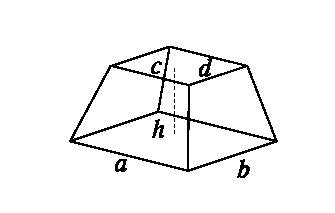
\includegraphics[width=0.5\textwidth]{guterStartInsPraktikum/bilder/obelisk}
\end{center}

%  \item Schreiben Sie ein Java-Programm, welches das Kugelvolumen einer beliebigen Kugel berechnet
% \end{itemize}
% \smallskip
%
% Ben"otigte Werkzeuge:
% \begin{itemize}
%  \item Standard Programmierger"ust
%  \item Geeignete Variablen f"ur $r$ und $v$
%  \item Einlesen von Variablen
%  \item Wert von $\pi$
%  \item Ausgeben des Ergebnisses
% \end{itemize}
\end{frame}

\begin{frame}[t]%
    \frametitle{\kap.\ref{S:Beispiel Obelisk} \stitle}%
\medskip
Dann ist:
\begin{itemize}
\item $G_1 = ab$ der Fl\"acheninhalt der Grundfl\"ache.
\item $G_2 = cd$ der Fl\"acheninhalt der Deckfl\"ache.
\item $\displaystyle A_1 = \frac{a+c}{2} \sqrt{h^2 + \Bigl(\frac{b-d}{2}\Bigr)^2}$
der Fl\"acheninhalt zweier Mantelfl\"achen.
\item $\displaystyle A_2 = \frac{b+d}{2} \sqrt{h^2 + \Bigl(\frac{a-c}{2}\Bigr)^2}$
der Fl\"acheninhalt der anderen beiden Mantelfl\"achen.
\item $M = 2 A_1 + 2 A_2$ der Fl\"acheninhalt der gesamten Mantelfl\"ache.
\item $O = M + G_1 + G_2$ der Fl\"acheninhalt der Oberfl\"ache .
\item $\displaystyle V = \frac{h}{6}\bigl(G_1 + (a+c)(b+d) + G_2\bigr)$ das Volumen.
\end{itemize}
\medskip

Schreiben Sie ein Java--Programm, welches die Seitenl\"angen $a$, $b$, $c$ und $d$ sowie
die H\"ohe $h$ eines Obelisken von der Konsole einliest und anschlie\ss end den Fl\"acheninhalt
der Mantelfl\"ache $M$, den der Oberfl\"ache $O$ sowie das Volumen $V$ ausgibt.

\end{frame}

\begin{frame}[t]%
    \frametitle{\kap.\ref{S:Beispiel Obelisk} \stitle}%
\medskip


\codeblock{\noindent
\cmt{
/* Berechnung von\\
\ * \ Mantelflaeche M\\
\ * \ Oberflaeche O\\
\ * \ Volumen V\\
\ * eines Obelisken\\
\ * \\
\ * Eingabe: a,b,c,d (Seitenlaengen) h (Hoehe)\\
\ * Ausgabe: M, O, V\\
\ * Author: Stefan Findeisen 2016\\
\ */\\[1em]
 }
public class Obelisk \{\\
\tab public static void main(String[] args) \{\\
\tab \tab \cmt{/* Hier steht das Hauptprogramm */}\\
\tab \tab ...\\
\tab \}\\
\}\\
}
\end{frame}

\begin{frame}[t]%
    \frametitle{\kap.\ref{S:Beispiel Obelisk} \stitle}%
\medskip

\codeblock{\noindent
\cmt{
/* Berechnung von\\
\ * \ Mantelflaeche M\\
\ * \ Oberflaeche O\\
\ * \ Volumen V\\
\ * eines Obelisken\\
\ * \\
\ * Eingabe: a,b,c,d (Seitenlaengen) h (Hoehe)\\
\ * Ausgabe: M, O, V\\
\ * Author: Stefan Findeisen 2016\\
\ */\\[1em]
 }
public class Obelisk \{\\
\tab public static void main(String[] args) \{\\
\tab \tab \cmt{/* Hier steht das Hauptprogramm */}\\
\tab \tab \cmt{/* Setze die Standardeinstellungen */}\\
\tab \tab {\color{red} Locale.setDefault(Locale.US);}\\
\tab \tab ...\\
\tab \}\\
\}\\
}
\end{frame}

\begin{frame}[t]%
    \frametitle{\kap.\ref{S:Beispiel Obelisk} \stitle}%
\medskip

\codeblock{\noindent
\cmt{
\ ...\\
\ * Eingabe: a,b,c,d (Seitenlaengen) h (Hoehe)\\
\ * Ausgabe: M, O, V\\
\ * Author: Stefan Findeisen 2016\\
\ */\\[1em]
 }
public class Obelisk \{\\
\tab public static void main(String[] args) \{\\
\tab \tab \cmt{/* Hier steht das Hauptprogramm */}\\
\tab \tab \cmt{/* Setze die Standardeinstellungen */}\\
\tab \tab Locale.setDefault(Locale.US);\\[1em]
\tab \tab \cmt{/* Daten des Obelisken */}\\
\tab \tab {\color{red} double a, b, c, d;} \cmt{// Seitenlaengen}\\
\tab \tab {\color{red} double h;} \cmt{ // Hoehe}\\
\tab \tab ...\\
\tab \}\\
\}\\
}
\end{frame}

\begin{frame}[t]%
    \frametitle{\kap.\ref{S:Beispiel Obelisk} \stitle}%
\medskip

\codeblock{\noindent
\cmt{...}\\[1em]
public class Obelisk \{\\
\tab public static void main(String[] args) \{\\
\tab \tab \cmt{/* Hier steht das Hauptprogramm */}\\
\tab \tab \cmt{/* Setze die Standardeinstellungen */}\\
\tab \tab Locale.setDefault(Locale.US);\\[1em]
\tab \tab \cmt{/* Daten des Obelisken */}\\
\tab \tab {\color{red} double a, b, c, d;} \cmt{// Seitenlaengen}\\
\tab \tab {\color{red} double h;} \cmt{ // Hoehe}\\[1em]
\tab \tab \cmt{/* Eingabe */}\\
\tab \tab \cmt{/* Hilfstext: */}\\
\tab \tab {\color{red} System.out.println(''Geben Sie die Seitenlaengen (a,b,c,d) '' +\\
\tab \tab \tab         ''sowie die Hoehe h eines Obelisken ein:'');}\\
\tab \tab ...\\
\tab \}\\
\}\\
}
\end{frame}

\begin{frame}[t]%
    \frametitle{\kap.\ref{S:Beispiel Obelisk} \stitle}%
\vspace{-1em}
\codeblock{\noindent
public class Obelisk \{\\
\tab public static void main(String[] args) \{\\
\tab \tab ...\\
\tab \tab \cmt{/* Eingabe */}\\
\tab \tab \cmt{/* Hilfstext: */}\\
\tab \tab System.out.println(''Geben Sie die Seitenlaengen (a,b,c,d) '' +\\
\tab \tab \tab         ''sowie die Hoehe h eines Obelisken ein:'');\\
\tab \tab \cmt{/* Eigentliche Eingabe mit Hilfstexten */}\\
\tab \tab {\color{red} Scanner sc = new Scanner(System.in);\\
\tab \tab   System.out.print(''a = '');\\
\tab \tab   a = sc.nextDouble();\\
\tab \tab   System.out.print(''b = '');\\
\tab \tab   b = sc.nextDouble();\\
\tab \tab   System.out.print(''c = '');\\
\tab \tab   c = sc.nextDouble();\\
\tab \tab   System.out.print(''d = '');\\
\tab \tab   d = sc.nextDouble();\\
\tab \tab   System.out.print(''h = '');\\
\tab \tab   h = sc.nextDouble();}\\
\tab \tab ...\\
\tab \}\\
\}\\
}
\end{frame}

\begin{frame}[t]%
    \frametitle{\kap.\ref{S:Beispiel Obelisk} \stitle}%

\codeblock{\noindent
{\color{red} import java.util.*;}  \cmt{// wird wegen ''Scanner'' benoetigt}\\[1em]
public class Obelisk \{\\
\tab public static void main(String[] args) \{\\
\tab \tab ...\\
\tab \tab \cmt{/* Eingabe */}\\
\tab \tab \cmt{/* Hilfstext: */}\\
\tab \tab System.out.println(''Geben Sie die Seitenlaengen (a,b,c,d) '' +\\
\tab \tab \tab         ''sowie die Hoehe h eines Obelisken ein:'');\\
\tab \tab \cmt{/* Eigentliche Eingabe mit Hilfstexten */}\\
\tab \tab {\color{red} Scanner sc = new Scanner(System.in);\\
\tab \tab   ...}\\
\tab \tab ...\\
\tab \}\\
\}\\
}
\end{frame}

\begin{frame}[t]%
    \frametitle{\kap.\ref{S:Beispiel Obelisk} \stitle}%

\codeblock{\noindent
import java.util.*;  \cmt{// wird wegen ''Scanner'' benoetigt}\\[1em]
public class Obelisk \{\\
\tab public static void main(String[] args) \{\\
\tab \tab ...\\
\tab \tab \cmt{/* Berechung */}\\
}
\begin{itemize}
\item $G_1 = ab$ Fl\"acheninhalt der Grundfl\"ache:
\end{itemize}
\codeblock{\noindent
\tab \tab {\color{red} double G1 = a * b;}\\
}
\begin{itemize}
\item $G_2 = cd$ Fl\"acheninhalt der Deckfl\"ache:
\end{itemize}
\codeblock{\noindent
\tab \tab {\color{red} double G2 = c * d;}\\
\tab \tab ...\\
\tab \}\\
\}\\
}
\end{frame}

\begin{frame}[t]%
    \frametitle{\kap.\ref{S:Beispiel Obelisk} \stitle}%

\codeblock{\noindent
import java.util.*;  \cmt{// wird wegen ''Scanner'' benoetigt}\\[1em]
public class Obelisk \{\\
\tab public static void main(String[] args) \{\\
\tab \tab ...\\
\tab \tab \cmt{/* Berechung */}\\
\tab \tab ...\\
}
\begin{itemize}
\item $\displaystyle A_1 = \frac{a+c}{2} \sqrt{h^2 + \Bigl(\frac{b-d}{2}\Bigr)^2}$
Fl\"acheninhalt zweier Mantelfl\"achen:
\end{itemize}
\codeblock{\noindent
\tab \tab {\color{red} double s1 = 0.5 * (a + c);\\
\tab \tab double t1 = 0.5 * (b - d);}\\
\tab \tab double A1 = s1 * Math.sqrt(h * h + t1 * t1);\\
}
\begin{itemize}
\item $\displaystyle A_2 = \frac{b+d}{2} \sqrt{h^2 + \Bigl(\frac{a-c}{2}\Bigr)^2}$
Fl\"acheninhalt der anderen Mantelfl\"achen:
\end{itemize}
\codeblock{\noindent
\tab \tab {\color{red} double s2 = 0.5 * (b + d);\\
\tab \tab double t2 = 0.5 * (a - c);}\\
\tab \tab double A2 = s2 * Math.sqrt(h * h + t2 * t2);\\
\tab \tab ...\\
\tab \}\\
\}\\
}
\end{frame}

\begin{frame}[t]%
    \frametitle{\kap.\ref{S:Beispiel Obelisk} \stitle}%

\codeblock{\noindent
import java.util.*;  \cmt{// wird wegen ''Scanner'' benoetigt}\\[1em]
public class Obelisk \{\\
\tab public static void main(String[] args) \{\\
\tab \tab ...\\
\tab \tab \cmt{/* Berechung */}\\
\tab \tab ...\\
}
\begin{itemize}
\item $\displaystyle A_1 = \frac{a+c}{2} \sqrt{h^2 + \Bigl(\frac{b-d}{2}\Bigr)^2}$
Fl\"acheninhalt zweier Mantelfl\"achen:
\end{itemize}
\codeblock{\noindent
\tab \tab double s1 = 0.5 * (a + c);\\
\tab \tab double t1 = 0.5 * (b - d);\\
\tab \tab double A1 = s1 * {\color{red} Math.sqrt}(h * h + t1 * t1);\\
}
\begin{itemize}
\item $\displaystyle A_2 = \frac{b+d}{2} \sqrt{h^2 + \Bigl(\frac{a-c}{2}\Bigr)^2}$
Fl\"acheninhalt der anderen Mantelfl\"achen:
\end{itemize}
\codeblock{\noindent
\tab \tab double s2 = 0.5 * (b + d);\\
\tab \tab double t2 = 0.5 * (a - c);\\
\tab \tab double A2 = s2 * {\color{red} Math.sqrt}(h * h + t2 * t2);\\
\tab \tab ...\\
\tab \}\\
\}\\
}
\end{frame}

\begin{frame}[t]%
    \frametitle{\kap.\ref{S:Beispiel Obelisk} \stitle}%

\codeblock{\noindent
import java.util.*;  \cmt{// wird wegen ''Scanner'' benoetigt}\\[1em]
public class Obelisk \{\\
\tab public static void main(String[] args) \{\\
\tab \tab ...\\
\tab \tab \cmt{/* Berechung */}\\
\tab \tab ...\\
}
\begin{itemize}
 \item $M = 2 A_1 + 2 A_2$ Fl\"acheninhalt der gesamten Mantelfl\"ache:
\end{itemize}
\codeblock{\noindent
\tab \tab {\color{red} double M = 2 * A1 + 2 * A2;}\\
}
\begin{itemize}
 \item $O = M + G_1 + G_2$ Fl\"acheninhalt der Oberfl\"ache:
\end{itemize}
\codeblock{\noindent
\tab \tab {\color{red} double O = M + G1 + G2;}\\
}
\begin{itemize}
 \item $\displaystyle V = \frac{h}{6}\bigl(G_1 + (a+c)(b+d) + G_2\bigr)$ Volumen:
\end{itemize}
\codeblock{\noindent
\tab \tab {\color{red} double V = h / 6 * (G1 + (a + c) * (b + d) + G2);}\\
\tab \tab ...\\
\tab \}\\
\}\\
}
\end{frame}

\begin{frame}[t]%
    \frametitle{\kap.\ref{S:Beispiel Obelisk} \stitle}%

\codeblock{\noindent
import java.util.*;  \cmt{// wird wegen ''Scanner'' benoetigt}\\[1em]
public class Obelisk \{\\
\tab public static void main(String[] args) \{\\
\tab \tab ...\\
\tab \tab \cmt{/* Ausgabe */}\\
\tab \tab {\color{red} System.out.println(''Mantelflaeche = '' + M);\\
\tab \tab System.out.println(''Oberflaeche = '' + O);\\
\tab \tab System.out.println(''Volumen = '' + V);}\\
\tab \}\\
\}\\
}
\end{frame}

\begin{frame}[t]%
    \frametitle{\kap.\ref{S:Beispiel Obelisk} \stitle}%
\tiny
\codeblock{\noindent
import java.util.*; \cmt{// wird wegen ''Scanner'' benoetigt}\\[1em]
\cmt{
/* Berechnung von Mantelflaeche M, Oberflaeche O, Volumen V, eines Obelisken\\
 * Eingabe: a,b,c,d (Seitenlaengen) h (Hoehe)\\
 * Ausgabe: M, O, V\\
 * Author: Stefan Findeisen 2016\\
 */}\\[1em]
public class Obelisk \{\\
\tab public static void main(String[] args) \{\\
\tab \tab \cmt{/* Hier steht das Hauptprogramm */}\\
\tab \tab \cmt{/* Setze die Standardeinstellungen */}\\
\tab \tab Locale.setDefault(Locale.US);\\[1em]
\tab \tab \cmt{/* Daten des Obelisken */}\\
\tab \tab double a, b, c, d; \cmt{// Seitenlaengen}\\
\tab \tab double h; \cmt{// Hoehe}\\
\tab \tab \cmt{/* Eingabe */\\
\tab \tab /* Hilfstext: */}\\
\tab \tab System.out.println(''Geben Sie die Seitenlaengen (a,b,c,d) '' +\\
\tab \tab \tab ''sowie die Hoehe h eines Obelisken ein:'');\\[1em]
\tab \tab \cmt{/* Eigentliche Eingabe mit Hilfstexten */}\\
\tab \tab Scanner sc = new Scanner(System.in);\\[1em]
\tab \tab System.out.print(''a = '');\\
\tab \tab a = sc.nextDouble();\\
\tab \tab System.out.print(''b = '');\\
\tab \tab b = sc.nextDouble();\\
\tab \tab System.out.print(''c = '');\\
\tab \tab c = sc.nextDouble();\\
\tab \tab System.out.print(''d = '');\\
\tab \tab d = sc.nextDouble();\\
\tab \tab System.out.print(''h = '');\\
\tab \tab h = sc.nextDouble();\\
\tab \tab ...\\
\tab \}\\
\}
}
\end{frame}

\begin{frame}[t]%
    \frametitle{\kap.\ref{S:Beispiel Obelisk} \stitle}%
\tiny
\codeblock{\noindent
import java.util.*; \cmt{// wird wegen ''Scanner'' benoetigt}\\[1em]
\cmt{
/* Berechnung von Mantelflaeche M, Oberflaeche O, Volumen V, eines Obelisken\\
 * Eingabe: a,b,c,d (Seitenlaengen) h (Hoehe)\\
 * Ausgabe: M, O, V\\
 * Author: Stefan Findeisen 2016\\
 */}\\[1em]
public class Obelisk \{\\
\tab public static void main(String[] args) \{\\
\tab \tab \cmt{/* Hier steht das Hauptprogramm */}\\
\tab \tab ...\\
\tab \tab \cmt{/* Berechung */}\\
\tab \tab double G1 = a * b;\\
\tab \tab double G2 = c * d;\\
\tab \tab double s1 = 0.5 * (a + c);\\
\tab \tab double s2 = 0.5 * (b + d);\\
\tab \tab double t1 = 0.5 * (b - d);\\
\tab \tab double t2 = 0.5 * (a - c);\\
\tab \tab double A1 = s1 * Math.sqrt(h * h + t1 * t1);\\
\tab \tab double A2 = s2 * Math.sqrt(h * h + t2 * t2);\\[1em]
\tab \tab double M = 2 * A1 + 2 * A2;\\
\tab \tab double O = M + G1 + G2;\\
\tab \tab double V = h / 6 * (G1 + (a + c) * (b + d) + G2);\\[1em]
\tab \tab \cmt{/* Ausgabe */}\\
\tab \tab System.out.println(''Mantelflaeche = '' + M);\\
\tab \tab System.out.println(''Oberflaeche = '' + O);\\
\tab \tab System.out.println(''Volumen = '' + V);\\
\tab \}\\
\}
}
\end{frame}



\begin{frame}
  \frametitle{Zusammenfassung}%
\tableofcontents[current]
\end{frame}

%%%%%%%%%%%%%%%%%%%%%%%%%%%%%%%%%%%%%%%%%%%%%%%%%%%%%%%%%%%%%%%%%%%%%%%%
\begin{frame}
\centering
\Huge\textcolor{KITgreen}{Fragen?}
\vspace{2cm}

{\LARGE
N\"achste \"Ubung: 30. November\\
Besprechung Arbeitsblatt 2
}
\end{frame}


%%%%%%%%%%%%%%%%%%%%%%%%%%%%%%%%%%%%%%%%%%%%%%%%%%%%%%%%%%%%%%%%%%%%%%%%
\end{document}
